\documentclass%
%[handout]
{beamer}
% % % % % % % %
% % % % % % % %
% % % % % % % %
%IMPORTANT
%compiles with 
%pdflatex -shell-escape 
%IMPORTANT
% % % % % % % %
% % % % % % % %
% % % % % % % %
\mode<presentation>
{
\useinnertheme{rounded}
\useoutertheme{infolines}
\usecolortheme{orchid}
\usecolortheme{whale}
}

\usepackage[english]{babel}
\usepackage[latin1]{inputenc}
\usepackage[all,cmtip]{xy}
\usepackage{times}
\usepackage[T1]{fontenc}
\usepackage{../example-templates}
\usepackage{../pstricks-commands}
\usepackage{cancel}

\usepackage{auto-pst-pdf}
\usepackage{pst-plot}
%\usepackage{pstricks-add} 

% Or whatever. Note that the encoding and the font should match. If T1
% does not look nice, try deleting the line with the fontenc.

\graphicspath{{../../modules/}}

\newtheoremstyle{partialproof}{3pt}{3pt}{}{}{}{.}{.5em}{}
\theoremstyle{partialproof} \newtheorem{partialproof}[theorem]{Proof.}
%\DeclareMathOperator{\diff}{d}
\newcommand{\diff}{\text{d}}
\setbeamertemplate{navigation symbols}{}

\includeonlylecture{1}

\newcommand{\lect}[3]{
  \date{#1}
  \lecture[#1]{#2}{#3}
}

\setbeamertemplate{footline}
{
  \leavevmode%
  \hbox{%
  \begin{beamercolorbox}[wd=.333333\paperwidth,ht=2.25ex,dp=1ex,center]{author in head/foot}%
    \usebeamerfont{author in head/foot}\insertshortauthor
  \end{beamercolorbox}%
  \begin{beamercolorbox}[wd=.333333\paperwidth,ht=2.25ex,dp=1ex,center]{title in head/foot}%
    \usebeamerfont{title in head/foot}\insertshorttitle
  \end{beamercolorbox}%
  \begin{beamercolorbox}[wd=.333333\paperwidth,ht=2.25ex,dp=1ex,center]{date in head/foot}%
    \usebeamerfont{date in head/foot}\insertshortdate{}
  \end{beamercolorbox}}%
  \vskip0pt%
}

% If you have a file called "university-logo-filename.xxx", where xxx
% is a graphic format that can be processed by latex or pdflatex,
% resp., then you can add a logo as follows:

%\pgfdeclareimage[height=0.8cm]{logo}{bluelogo}
%\logo{\pgfuseimage{logo}}

\begin{document}

\AtBeginLecture{%

\title[\insertlecture]{FreeCalc}
\subtitle{\insertlecture}
\author[FreeCalc]{}
\institute[UMass Boston]{University of Massachusetts Boston}
\date{\insertshortlecture}
\begin{frame}
  \titlepage
\end{frame}
}%

% begin lecture
\lect{\today}{Sample}{1}
%% begin module derivatives-rules-summary
\begin{frame}
\frametitle{Rules of differentiation.}
We studied the basic rules of differentiation.
\begin{itemize}
\item<1->\alertNoH{12}{ $f (g(x))'=f'(g(x)) g'(x) $ (Chain rule). }
\item<2->\alertNoH{12}{ $(f*g)'=f'g+fg'$ (Product rule).}
\item<3->\alertNoH{12}{ $(f+g)'=f'+g'$ (Sum rule). }
\item<4->\alertNoH{12}{ $x'=1$. }
\item<5->\alertNoH{12}{ $(c)'=0$ if $c$ is a constant (Constant derivative rule).}
\end{itemize}
\uncover<6->{We studied additional differentiation rules.}
\begin{itemize}
\item<6->\alertNoH{13}{ $(e^x)'=e^x$ (Exponent derivative rule).}
\item<7->\alertNoH{13}{ $\left(\frac{f}{g}\right)'=\frac{f' g-f g' }{g^2}$ (Quotient rule).}
\item<8->\alertNoH{13}{ $(x^r)'=rx^{r-1} $, $r$-arbitrary real number (Power rule).}
\item<9->\alertNoH{13}{ $(\ln x)'=\frac{1}x$ (Logarithm derivative rule). }
\item<10->\alertNoH{13}{ $(\log_a x)'=\frac{1}{x\ln a}$.}
\item<11->\alertNoH{13}{ $(\sin x)'=\cos x$, $(\cos x)'=-\sin x$}
\end{itemize}

\uncover<12->{We derived \alertNoH{12}{the first set of rules}  by directly computing limits. } \uncover<13->{The \alertNoH{13}{second set of rules} can be derived from the first set \uncover<13>{algebraically}.}
\end{frame}
% end module derivatives-rules-summary

%% begin module power-rule-from-exponent
\begin{frame}
\begin{example}
Let $c$ be a constant. Derive the constant multiple rule 
\[
\alert<6>{(cf)'=c f'}
\]
\uncover<3->{using the \alert<3>{product rule $(fg)'=f'g+fg'$}} \uncover<4->{\alert<4>{and the constant derivative rule $(c)'=0$.}}

\[
\uncover<2->{\alert<3,6>{(cf)'}=} \uncover<3->{\alert<3>{\alert<4>{(c)'} f+ c f'}=}\uncover<4->{\alert<4>{0} f+cf'=}\uncover<5->{\alert<6>{cf'}}
\]
\uncover<6->{\alert<6>{as desired}.}
\end{example}

\end{frame}

%end module power-rule-from-exponent
%% begin module derivatives-rules-relations

\begin{frame}
\begin{example}
Let $n$-positive integer. Derive the positive integer power rules
\[
\alertNoH{5,8}{\left( x^2\right)' =2x }, \quad \quad
\alertNoH{9,12}{\left( x^3\right)' =3x^2}, \quad \quad \alertNoH{13}{\left( x^4\right)' =4x^3}, \quad \quad \alertNoH{19}{\dots}
\]
\uncover<2->{\alertNoH{2}{using the rule $(x)'=1$}} \uncover<4->{\alertNoH{4,7,11,16}{and the product rule}.}

\[
\begin{array}{rcl}
\uncover<2->{\alertNoH{2}{(x)'}&=&\alertNoH{2}{1}}\\
\uncover<3->{\alertNoH{5,8}{(x^2)'}&=& \alertNoH{4}{(x\cdot x)'} = \uncover<4->{\alertNoH{4}{x'x +x x'}=} \uncover<5->{x+x=\alertNoH{5,8}{2x} }} \\
\uncover<6->{\alertNoH{9,12}{(x^{3})'}&=& \alertNoH{7}{(x\cdot x^2)'}=} \uncover<7->{\alertNoH{7}{x' x^2+x\alertNoH{8}{(x^2)'}}=} \uncover<8->{x^2+ x (\alertNoH{8}{2x})=} \uncover<9->{x^2+2x^2= \alertNoH{9,12}{3x^2}}\\
\uncover<10->{\alertNoH{13}{(x^{4})'}&=& \alertNoH{11}{(x\cdot x^3)'}=\uncover<11->{\alertNoH{11}{x' x^3+x\alertNoH{12}{(x^3)'}}=} \uncover<12->{ x^3+ x (\alertNoH{12}{3x^2})=}\uncover<13->{x^3+3x^3=\alertNoH{13}{4x^3}}}\\
\uncover<14->{&\vdots&}\\
\uncover<15->{\alertNoH{17}{(x^{n})'}&=&\dots = \alertNoH{17}{n x^{n-1}}}\\
\uncover<15->{\alertNoH{18}{ (x^{n+1})'}&=&\alertNoH{16}{(x\cdot x^n)'}=}\uncover<16->{\alertNoH{16}{ x' x^n+ x \alertNoH{17}{(x^{n})'}}=} \uncover<17->{x^n+x (\alertNoH{17}{nx^{n-1}})=} \uncover<18->{\alertNoH{18}{(n+1)x^n}}\\
\uncover<19->{&\alertNoH{19}{\vdots}&}
\end{array}
\]
\end{example}


\end{frame}




%end module derivatives-rules-relations

%% begin module derivatives-rules-relations

\begin{frame}
\begin{example}
Let $n$ be a positive integer. Derive the negative integer power rule
\[
(x^{-n})'=\left(\frac{1}{x^n}\right)'= -n x^{-n-1} =-\frac{n}{x^{n+1}}
\]
\uncover<4->{using \alertNoH{4}{the product rule},} \uncover<5->{\alertNoH{5}{the constant derivative rule}} \uncover<6->{and \alertNoH{6}{the power rule for positive integers}.}

\[
\begin{array}{rcl p{2cm} |r}
\uncover<2->{ x^n x^{-n} &=& 1  &&} \uncover<3->{\frac{d}{dx}}\\
\uncover<3->{\alertNoH{4}{( x^n x^{-n})'} &=&\alertNoH{5}{(1)'}  }\\

\uncover<4->{ \alertNoH{4}{ \alertNoH{6}{(x^n)'} x^{-n} + x^n (x^{-n})'}&=&\alertNoH{5}{0}}\\
\uncover<6->{ \alertNoH{7}{\alertNoH{6}{n x^{n-1}}x^{-n}}+ x^n (x^{-n})'&=&0 }\\
\uncover<7->{\alertNoH{7}{\frac{n}{x}}+ x^n (x^{-n})'&=&0 }\\
\uncover<8->{x^n (x^{-n})'&=&-\frac{n}x && \frac{1}{x^n}}\\
\uncover<9->{(x^{-n})'&=&-\frac{n}{x^{n+1}}}
\end{array}
\]

\end{example}



\end{frame}




%end module derivatives-rules-relations

%% begin module power-rule-rationa-from-chain-rule
\begin{frame}
\begin{example}
Derive the power rule $\alertNoH{13}{\left(x^{\frac{1}{q}}\right)'=\frac{1}{q} x^{\frac{1}q-1}}$ \uncover<4->{using \alertNoH{4}{the rule $(x)'=1$},} \uncover<6->{\alertNoH{6}{the chain rule}} \uncover<7->{and the \alertNoH{7}{integer power rule $\frac{d}{du}(u^q)=qu^{q-1} $}.}

\[
\begin{array}{rclp{0.3cm}|l}
\uncover<2->{ \left(x^{\frac{1}{q}}\right)^q &=&x&& \uncover<3->{\alertNoH{3}{\frac{d}{dx}}}}\\
\uncover<3->{ \alertNoH{3}{\left(\left(\alertNoH{5}{x^{\frac{1}q}} \right)^q\right)'} &=& \uncover<4->{\alertNoH{4}{1}} \uncover<3>{\alertNoH{3}{(x)'}} &&\uncover<5->{\alertNoH{5,8}{\text{Set~}u=x^{\frac1q} }}}\\
\uncover<5->{ \alertNoH{6}{\left(\alertNoH{5}{u}^{q}\right)'}&=&1  }  \\
\uncover<6->{\alertNoH{6}{ \alertNoH{7}{\frac{d}{du} \left(u^q\right)} u'}&=&1}\\
\uncover<7->{\alertNoH{7}{q (\alertNoH{8}{u})^{q-1}} (\alertNoH{8}{u})'&=&1 }\\
\uncover<8->{ q (\alertNoH{8}{x^{\alertNoH{9}{\frac{1}q}}})^{\alertNoH{9}{q-1}} \left( \alertNoH{8}{x^{\frac1q}}\right)'&=&1 }\\
\uncover<9->{\alertNoH{10}{q x^{\alertNoH{9}{\frac{q-1}q}}}\left( x^{\frac1q}\right)'&=&1&&\uncover<10->{\alertNoH{10}{\text{divide~by~}q x^{\frac{q-1}q}}}}\\
\uncover<10->{\alertNoH{13}{\left( x^{\frac1q}\right)'}&=&\frac{ 1}{\alertNoH{10}{q \alertNoH{11}{x^{\frac{q-1}q}}}}= \uncover<11->{ \frac{\alertNoH{11}{x^{\alertNoH{12}{-\frac{q-1}{q}}}}}{q}=}\uncover<12->{\alertNoH{13}{\frac{1}q x^{\alertNoH{12}{\frac{1}q-1}}}} &&\uncover<13->{\alertNoH{13}{\text{as~desired}}}}
\end{array}
\]
\end{example}

\end{frame}

%end module power-rule-rationa-from-chain-rule

%% begin module quotient-rule-from-power-and-chain
\begin{frame}
\begin{example}
Derive the quotient rules
\[
\begin{array}{rcl}
\alertNoH{5,9}{\displaystyle\left(\frac{1}{g}\right)'}&=&\displaystyle\alertNoH{5,9}{-\frac{g'}{g^2}}
\\
\displaystyle\alertNoH{11}{\left(\frac{f}{g}\right)'}&=&\displaystyle\alertNoH{11}{\frac{f'g-fg'}{g^2}}
\end{array}
\]
\uncover<3->{using \alertNoH{3}{the chain rule},} \uncover<4->{\alertNoH{4}{the negative power rule}} \uncover<8->{and \alertNoH{8}{the product rule}.}
\[
\begin{array}{rclp{0.3cm}|l}
\displaystyle \uncover<2->{ \alertNoH{3,5}{\left(\frac{1}{g}\right)'} &=&\displaystyle \uncover<3->{\alertNoH{3}{\alertNoH{4}{\frac{d}{dg}\left(\frac1g\right)} g'}=}\uncover<4->{\alertNoH{5}{\alertNoH{4}{-\frac{1}{g^2}}g'}}&&\uncover<5->{\alertNoH{5}{\text{as~desired}}}}\\
\\
\displaystyle
\uncover<6->{\alertNoH{7,11}{\left(\frac{f}{g}\right)'}\uncover<7->{&=&\displaystyle\alertNoH{7,8}{\left( f \frac{1}g\right)'}=}\uncover<8->{\alertNoH{8}{f' \frac{1}{g} +f\alertNoH{9}{\left(\frac{1}g\right)'}}=}\uncover<9->{\alertNoH{10}{\frac{f'}{g}+f\alertNoH{9}{\left(-\frac{g'}{g^2}\right)}}}}\\
\\
\uncover<10->{&=&\displaystyle
%\frac{f'g}{g^2} - \frac{fg'}{g^2}=
\alertNoH{10,11}{\frac{f'g-fg'}{g^2}} &&\uncover<11->{\alertNoH{11}{\text{as~desired}}}}
\end{array}
\]
\end{example}
\end{frame}
%end module quotient-rule-from-power-and-chain

%% begin module power-rule-rationa-from-chain-rule
\begin{frame}

\begin{example}
Derive \alert<11>{the exponent rule $\left(e^x\right)'=e^x$} \uncover<2->{using the Calc II formula below,} \uncover<3->{ \alert<3>{the infinite} {\color{gray!50} (both sides uniformly convergent)} \alert<3>{sum rule $(f_1+f_2 +f_3 +\dots)' =f_1' +f_2'  +f_3' +\dots$}}
\uncover<4->{and \alert<4>{the power rule $(x^n)'=nx^{n-1}$}. } 
\uncover<2->{\[
\alert<2,10>{e^x}=\alert<2,10>{1+x+\frac{x^2}{2!}+\frac{x^3}{3!}+\dots},
\]
}
\uncover<2->{where $n!=1\cdot2\cdot3\cdot \dots\cdot n$.} \uncover<5->{We have that $\alert<5,9>{\frac{n}{\alert<6>{ n!}}} =\uncover<6->{ \frac{\alert<7>{n} }{ \alert<6>{ 1\cdot 2\cdot \dots\cdot (n-1) \cdot  \alert<7>{n}}}=}\uncover<7->{\frac{1}{\alert<8>{1\cdot 2\cdot \dots\cdot (n-1)}}=}\uncover<8->{\alert<9>{ \frac{1}{ \alert<8>{(n-1)!} }}} $.}
\[
\begin{array}{rcl}
\uncover<2->{\alert<11>{\left(\alert<2>{e^x}\right)'} &=&\alert<3>{\left(\alert<2>{1+x+\frac{x^2}{2!}+\frac{x^3}{3!}+\dots} \right)' }} \\
\uncover<3->{&=& \alert<3>{ \alert<4>{(1)'}+\alert<4>{(x)'}+\frac{\alert<4>{(x^2)'}}{2!} +\frac{\alert<4>{(x^3)'}}{3!}+\dots + \frac{\alert<4>{(x^n)'}}{n!}+\dots}}
\\ \uncover<4->{&=&\alert<4>{0}+ \alert<4>{1}+ \frac{\alert<4>{\alert<5-9>{2}x}}{\alert<5-9>{2!}}+ \frac{\alert<4>{\alert<5-9>{3}x^2}}{\alert<5-9>{3!}}+ \dots +\frac{\alert<4>{\alert<5-9>{n}x^{n-1}}}{\alert<5-9>{n!}}+\dots }\\
\uncover<9->{&=& \alert<10>{ \phantom{ 0~ + }  1 + \frac{\phantom{2}x}{\alert<9>{1!}}+\frac{\phantom{3}x^{2}}{\alert<9>{2!}}+\dots+\frac{\phantom{n}x^{n-1}}{\alert<9>{(n-1)!}}+\dots}=}\uncover<10->{\alert<10,11>{e^x}}\\
\end{array}
\]
\uncover<11->{\alert<11>{as desired.}}
\end{example}

\end{frame}

%end module power-rule-rationa-from-chain-rule
%% begin module logarithm-rule-from-exponent
\begin{frame}
\begin{example}
Derive the logarithm derivative rules
\[
\begin{array}{rcl}
\alertNoH{11,15}{(\ln x)'}&=&\alertNoH{11,15}{\frac{1}{x}}\\
\alertNoH{16}{(\log_a x)'}&=&\alertNoH{16}{\frac{1}{x\ln a}}
\end{array}
\]
\uncover<5->{using \alertNoH{5}{the chain rule},} \uncover<6->{the \alertNoH{6}{exponent derivative rule $(e^{x})'=e^x$}, } \uncover<7->{\alertNoH{7}{the rule $(x)'=1$}} \uncover<14->{and the \alertNoH{14}{constant multiple rule $(cf)'=cf'$}.}
\[
\begin{array}{rclp{0.3cm}|l}
\uncover<2->{
e^{\alertNoH{3}{\ln x}}&=&x \uncover<3->{&&  \alertNoH{3,8}{ \text{set~~~}u =\ln x }}}\\
\uncover<3->{e^{\alertNoH{3}{u}}&=&x \uncover<4->{& & \alertNoH{4}{ \frac{\diff}{\diff x}}}}\\
\uncover<5->{ \alertNoH{5}{\alertNoH{6}{\frac{\diff}{\diff u}(e^u)} u'}&=&\alertNoH{7}{(x)'}}\\
\uncover<6->{ \alertNoH{6}{e^{\alertNoH{8}{u}}} \alertNoH{8}{u}'&=&\alertNoH{7}{1}}\\
\uncover<8->{\alertNoH{9}{e^{\alertNoH{8}{\ln x}}} (\alertNoH{8}{\ln x})'&=&1}\\
\uncover<9->{\alertNoH{9}{x}(\ln x)'&=&1\uncover<10->{& &\alertNoH{10}{ \cdot \frac{1}{x}}}}\\
\uncover<10->{ \alertNoH{11}{(\ln x)'} &=& \displaystyle\alertNoH{11}{\frac{1}x} \uncover<11->{ & &\alertNoH{11}{ \text{as~desired}}}} 
\uncover<12->{\\ \hline
\alertNoH{16}{(\alertNoH{13}{\log_a x})'} & =&  \uncover<13->{ \alertNoH{14}{\left(\alertNoH{13}{\frac{\ln x}{\ln a}} \right)' }=} \uncover<14->{\alertNoH{14}{ \frac{ \alertNoH{15}{ (\ln x)'}}{\ln a}} =} \uncover<14->{\alertNoH{16}{ \frac{ \alertNoH{15}{1} }{\alertNoH{15}{x}\ln a}}}\uncover<16>{ & &  \alertNoH{16}{ \text{as~desired~}}}}
\end{array}
\]
\end{example}
\end{frame}

%end module module logarithm-rule-from-exponent

%% begin module power-rule-from-exponent
\begin{frame}
\begin{example}

\end{example}

\end{frame}

%end module power-rule-from-exponent
%\section{Derivatives and the Shapes of Curves}
%\subsection{What Does $f''$ Say About $f$?}
%% begin module concavity-def
\begin{frame}
\frametitle{What Does $f''$ Say About $f$?}
$f$ and $g$ are both increasing on $(a,b)$, but ``bend'' in different directions.
\begin{columns}[c]
\column{.5\textwidth}
\psset{xunit=0.6cm, yunit=0.6cm}
\begin{pspicture}(-1,-1)(4,3.8)
\psframe*[linecolor=white](-1,-1)(4,3.8)
\psaxes[ticks=none, labels=none]{<->}(0,0)(-1,-1)(4,3.8)
%Function formula: 1/2+1/4 ((-1+x)^{2})+1/4 (x) =1/4x^{2}-1/4x +3/4
\psplot[linecolor=red, plotpoints=1000]{-1}{4}{x 0.25 mul x -1 add 2 exp 0.25 mul add 0.5 add }
\tiny
\rput(1, 2){$y=f(x)$}
\psXTickWithLabel{0.5}{$a$} 
\psXTickWithLabel{3.7}{$b$} 

\uncover<3>{ %point: x=0.3
%Function formula: -1/10 (x)+291/400 
\psplot[linecolor=blue, plotpoints=1000]{-0.5}{4}{0.7275 x -0.1 mul add }
}
\uncover<4->{%point: x=0.3
%Function formula: -1/10 (x)+291/400 
\psplot[linecolor=blue, plotpoints=1000]{0}{0.6}{0.7275 x -0.1 mul add } 
}
\uncover<3->{
\psFullDot{0.3}{0.6975}
}

\uncover<4>{ %point x=1.3
%Function formula: 2/5 (x)+131/400 
\psplot[linecolor=blue, plotpoints=1000]{-0.5}{4}{0.3275 x 0.4 mul add } 
}
\uncover<5->{ %point x=1.3
%Function formula: 2/5 (x)+131/400 
\psplot[linecolor=blue, plotpoints=1000]{1}{1.6}{0.3275 x 0.4 mul add } 
}
\uncover<4->{
\psFullDot{1.3}{0.8475}
}

\uncover<5>{ %point x=2.3
%Function formula: 9/10 (x)-229/400 
\psplot[linecolor=blue, plotpoints=1000]{0.080555556}{4}{-0.5725 x 0.9 mul add } 
}
\uncover<6->{ %point x=2.3
%Function formula: 9/10 (x)-229/400 
\psplot[linecolor=blue, plotpoints=1000]{2}{2.6}{-0.5725 x 0.9 mul add } 
}
\uncover<5->{
\psFullDot{2.3}{1.4975}
}

\uncover<6>{ %point x=3.3
%Function formula: 7/5 (x)-789/400 
\psplot[linecolor=blue, plotpoints=1000]{1.051785714}{4}{-1.9725 x 1.4 mul add } 
}
\uncover<7->{  %point x=3.3
%Function formula: 7/5 (x)-789/400 
\psplot[linecolor=blue, plotpoints=1000]{3}{3.6}{-1.9725 x 1.4 mul add } 
}
\uncover<6->{
\psFullDot{3.3}{2.6475}
}
\uncover<9>{
\psline[linecolor=blue](-1, 1.25) (1.6, 0.99)
}
\uncover<10->{
\psline[linecolor=blue!30](-1, 1.25) (1.6, 0.99)
}
\uncover<10>{
\psline[linecolor=blue](0, 0.75) (2.6, 1.79)
}
\uncover<11->{
\psline[linecolor=blue!30](0, 0.75) (2.6, 1.79)
}
\uncover<11>{
\psline[linecolor=blue](1, 0.75) (3.6, 3.09)
}
\uncover<12->{
\psline[linecolor=blue!30](1, 0.75) (3.6, 3.09)
}

\rput[t](2,-0.5) {\uncover<6->{Concave up}}
\end{pspicture} 
%\ \only<handout:0| -2>{%
%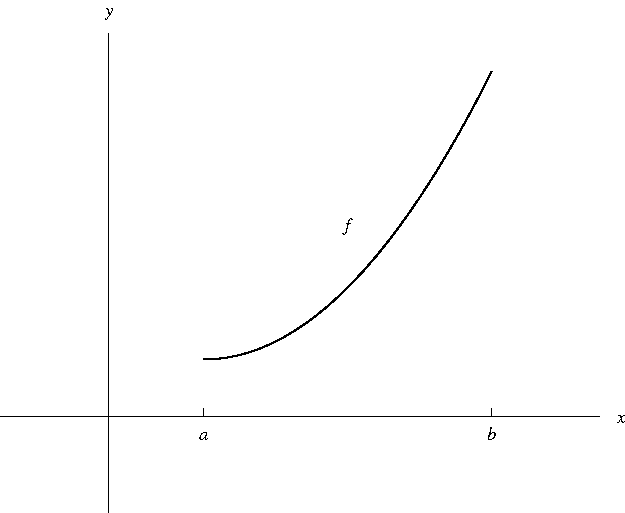
\includegraphics[height=3.5cm]{curve-sketching/pictures/04-03-concaveupa.pdf}%
%}%
%\only<handout:0| 3>{%
%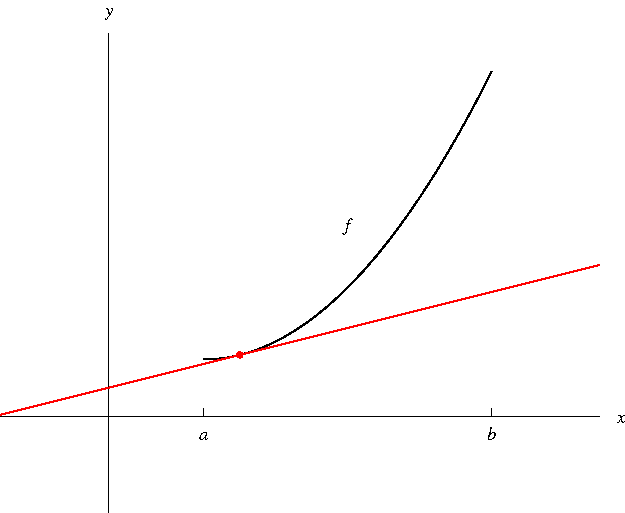
\includegraphics[height=3.5cm]{curve-sketching/pictures/04-03-concaveupb.pdf}%
%}%
%\only<handout:0| 4>{%
%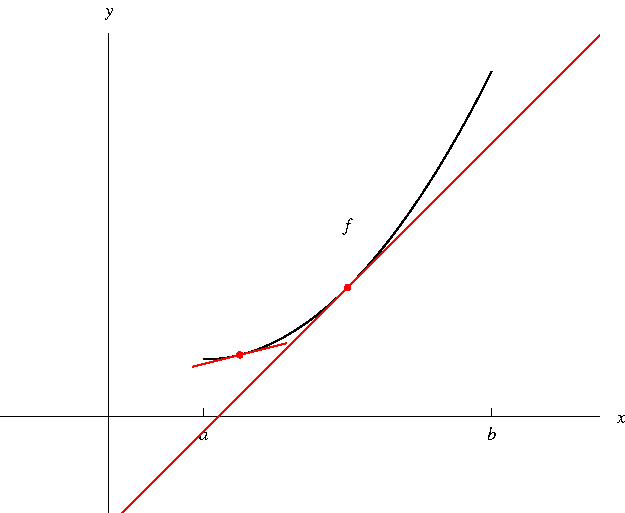
\includegraphics[height=3.5cm]{curve-sketching/pictures/04-03-concaveupc.pdf}%
%}%
%\only<handout:0| 5>{%
%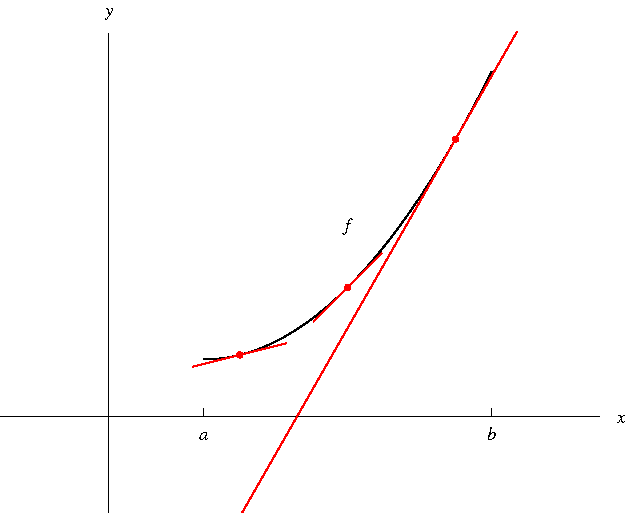
\includegraphics[height=3.5cm]{curve-sketching/pictures/04-03-concaveupd.pdf}%
%}%
%\only<6->{%
%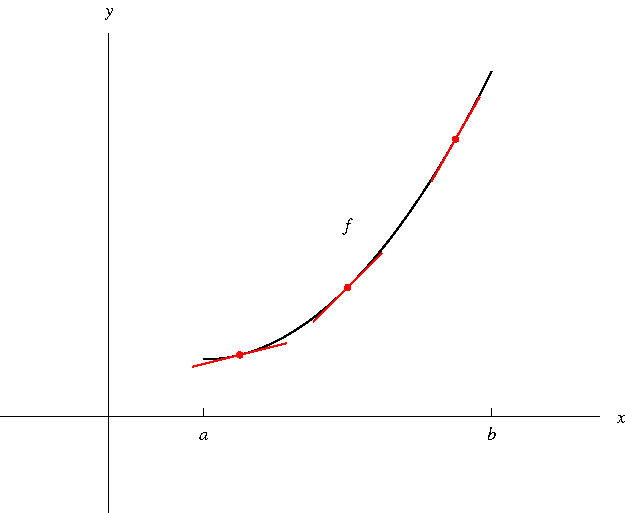
\includegraphics[height=3.5cm]{curve-sketching/pictures/04-03-concaveupe.pdf}%
%}%


\column{.5\textwidth}
\psset{xunit=0.6cm, yunit=0.6cm}
\begin{pspicture}(-1,-1)(4,3.8)
\psframe*[linecolor=white](-1,-1)(4,3.8)
\psaxes[ticks=none, labels=none]{<->}(0,0)(-1,-1)(4,3.8)
\tiny
\rput[l](2.5, 0.7){$y=g(x)$}
%Function formula: -1/4x^{2}+5/4x +1/2=11/4-1/4 (-3+x)^{2}-1/4 x 
\psplot[linecolor=red, plotpoints=1000]{-1}{4}{x -0.25 mul x -3 add 2 exp -0.25 mul add 2.75 add }
\psXTickWithLabel{0.3}{$a$} 
\psXTickWithLabel{2.5}{$b$} 


\uncover<3>{
%Function formula: 11/10 (x)+209/400 
\psplot[linecolor=blue, plotpoints=1000]{-0.5}{2.979}{0.5225 x 1.1 mul add }
}
\uncover<4->{ 
%Function formula: 11/10 (x)+209/400 
\psplot[linecolor=blue, plotpoints=1000]{0}{0.6}{0.5225 x 1.1 mul add } 
}
\uncover<3->{
\psFullDot{0.3}{0.8525}
}
\uncover<4>{
%Function formula: 3/5 (x)+369/400 
\psplot[linecolor=blue, plotpoints=1000]{-0.5}{4}{0.9225 x 0.6 mul add } 
}
\uncover<5->{
%Function formula: 3/5 (x)+369/400 
\psplot[linecolor=blue, plotpoints=1000]{1}{1.6}{0.9225 x 0.6 mul add } 
}
\uncover<4->{
\psFullDot{1.3}{1.7025}
}

\uncover<5>{
%Function formula: 1/10 (x)+729/400 
\psplot[linecolor=blue, plotpoints=1000]{-0.5}{4}{1.8225 x 0.1 mul add } 
}
\uncover<6->{
%Function formula: 1/10 (x)+729/400 
\psplot[linecolor=blue, plotpoints=1000]{2}{2.6}{1.8225 x 0.1 mul add } 
}
\uncover<5->{
\psFullDot{2.3}{2.0525}
}
\uncover<6>{
%Function formula: -2/5 (x)+1289/400 
\psplot[linecolor=blue, plotpoints=1000]{-0.5}{4}{3.2225 x -0.4 mul add } 
}
\uncover<7->{
%Function formula: -2/5 (x)+1289/400 
\psplot[linecolor=blue, plotpoints=1000]{3}{3.6}{3.2225 x -0.4 mul add } 
}
\uncover<6->{
\psFullDot{3.3}{1.9025}
}
\rput[t](2,-0.5) {\uncover<6->{Concave down}}
\uncover<9>{
\psline[linecolor=blue] (-1, -1) (1.6, 1.86)
}
\uncover<10->{
\psline[linecolor=blue!30] (-1, -1) (1.6, 1.86)
}
\uncover<10>{
\psline[linecolor=blue] (0, 0.5) (2.6, 2.06)
}
\uncover<11->{
\psline[linecolor=blue!30] (0, 0.5) (2.6, 2.06)
}
\uncover<11>{
\psline[linecolor=blue] (1, 1.5) (3.6, 1.76)
}
\uncover<12->{
\psline[linecolor=blue!30] (1, 1.5) (3.6, 1.76)
}

\end{pspicture} 
%\ \only<handout:0| -2>{%
%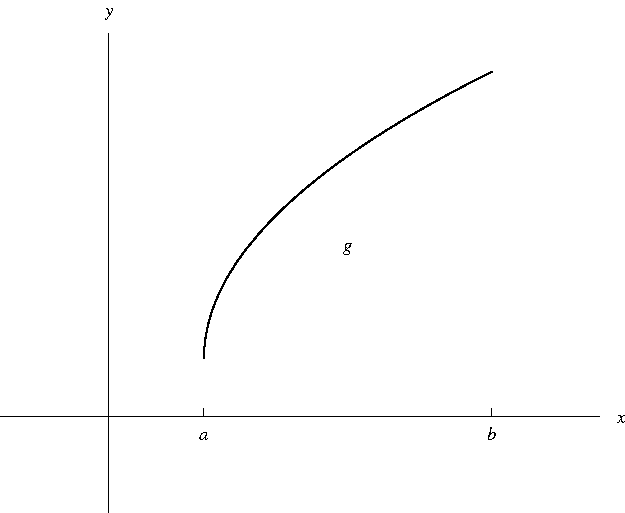
\includegraphics[height=3.5cm]{curve-sketching/pictures/04-03-concavedowna.pdf}%
%}%
%\only<handout:0| 3>{%
%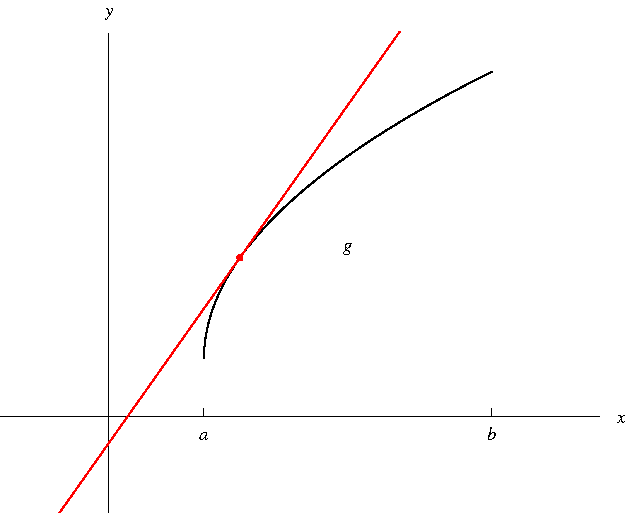
\includegraphics[height=3.5cm]{curve-sketching/pictures/04-03-concavedownb.pdf}%
%}%
%\only<handout:0| 4>{%
%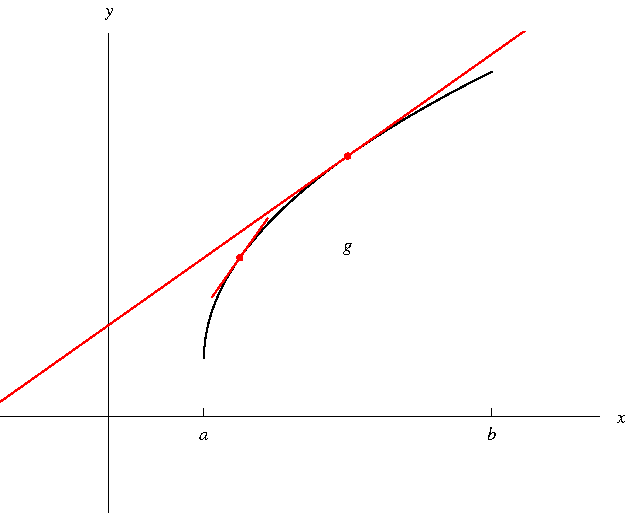
\includegraphics[height=3.5cm]{curve-sketching/pictures/04-03-concavedownc.pdf}%
%}%
%\only<handout:0| 5>{%
%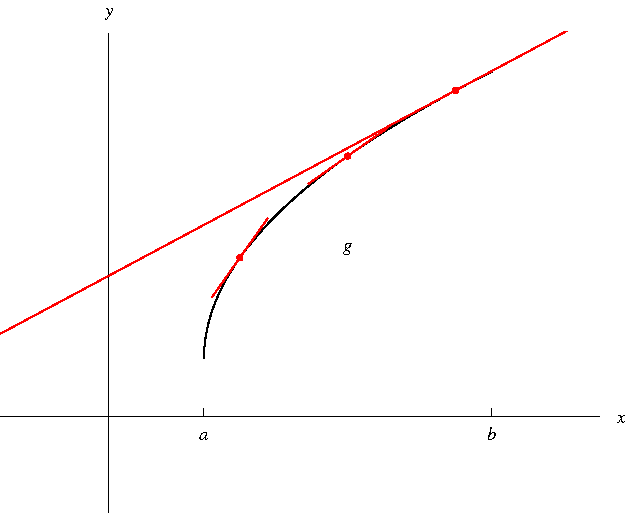
\includegraphics[height=3.5cm]{curve-sketching/pictures/04-03-concavedownd.pdf}%
%}%
%\only<6->{%
%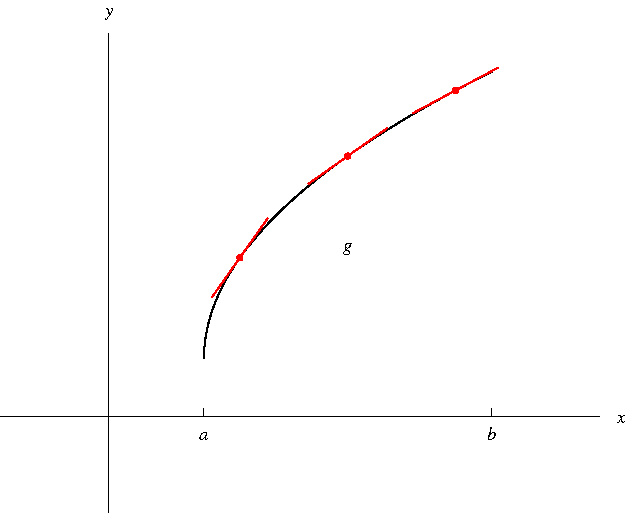
\includegraphics[height=3.5cm]{curve-sketching/pictures/04-03-concavedowne.pdf}%
%}%
\end{columns}
\uncover<8-12>{%
\begin{definition}[Concave Up/Concave Down, most general definition]
A function is called concave up/down if the line segment between any two points on its graph lies above/below the graph.
\end{definition}
}%
\uncover<2->{
\begin{theorem}[Can be taken as a definition]
Let $f$ be a differentiable function on an interval $I$. Then $f$ is
concave up (on $I$) if its graph lies above all of its tangents (on $I$), and $f$ is concave down (on $I$) if its graph lies below all of its tangents (on $I$).
\end{theorem}
}
\end{frame}
% end module concavity-def

%% begin module second-derivative-test
\begin{frame}
This gives us a new way of checking if critical points are local maxima or local minima:

\vspace{.3in}

The Second Derivative Test

Suppose $f''$ is exists near $c$.
\begin{enumerate}
\item  If $f'(c) = 0$ and $f''(c) > 0$, then $f$ has a local minimum at $c$.
\item  If $f'(c) = 0$ and $f''(c) < 0$, then $f$ has a local maximum at $c$.
\end{enumerate}
\uncover<2->{%
\begin{columns}[c]
\column{.3\textwidth}
\psset{xunit=1cm, yunit=1cm}
\begin{pspicture}(-0.5,-0.5)(3.4,2.7)
\tiny
\psaxes[ticks=none, labels=none]{<->}(0,0)(-0.5,-0.5)(3.3,2.6)
\fcLabels{3.3}{2.6}
%Function formula: -5/2-2 ((x) (x))+6 (x)
\psplot[linecolor=red, plotpoints=1000]{0.381966011}{2.618033989}{x 6 mul x x mul -2 mul add -2.5 add }
\psline[linestyle=dashed](1.5, 2)(1.5, 0)
\fcFullDot{1.5}{2}
\psline[linecolor=\fcColorTangent](-0.1,2)(2.9,2)
\tiny
\rput[t](1.5, -0.1){$c$}
\end{pspicture}

%\ 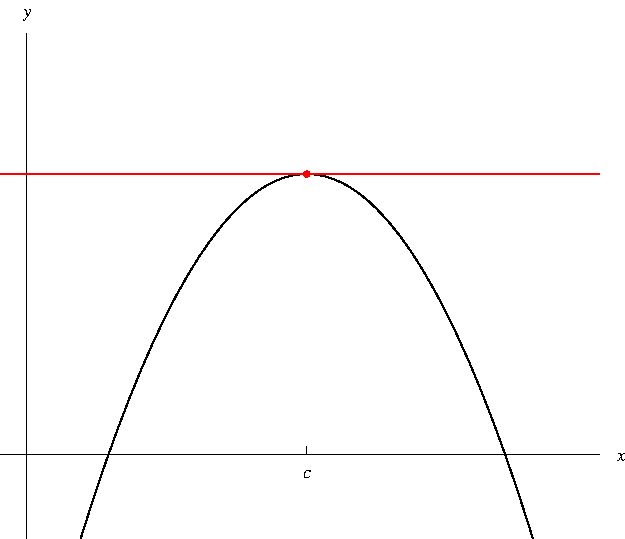
\includegraphics[height=3.5cm]{curve-sketching/pictures/04-03-secondderiv.pdf}%
\column{.7\textwidth}
\begin{itemize}
\item  $f'(c) = 0$, so $f$ has a horizontal tangent at $c$.
\item  $f''(c) < 0$, so $f$ is concave down near $c$.
\item  This means $f$ lies below its horizontal tangent.
\item  This means $f(c)$ is a local maximum.
\end{itemize}
\end{columns}
}%
\end{frame}
% end module second-derivative-test

%% begin module curve-sketching-ex6
\begin{frame}
\begin{example}
Discuss the curve $y = \alert<handout:0| 19-20,39-42>{f(x)}$ \alert<handout:0| 19-20,39-42>{$= x^4 - 4x^3$} with respect to \alert<handout:0| 28-35>{concavity}, \alert<handout:0| 36-42>{points of inflection}, and \alert<handout:0| 10-27>{local maxima and minima}.  \alert<handout:0| 43->{Sketch the curve.}
\begin{columns}[c]
\column{.42\textwidth}
\psset{xunit=0.8cm, yunit=0.1cm}
\begin{pspicture}(-1.2,-32)(4.4,10)
\psframe*[linecolor=white](-1.2,-32)(4.4,10)
\tiny
\psaxes[ticks=none, labels=none]{<->}(0,0)(-1.2,-30)(4.3,9)
\fcLabels{4.3}{9}
\fcYTickWithLabel{-10}{$-10$}
\fcYTickWithLabel{-20}{$-20$}
\fcYTickWithLabel{-30}{$-30$}
\psline(1, -0.8)(1,0.8)
\psline(2, -0.8)(2,0.8)
\psline(3, -0.8)(3,0.8)
\rput[t](1, -1.6){$1$}
\rput[t](2, -1.6){$2$}
\rput[t](3, -1.6){$3$}

%Function formula: (x)^{4}-4 ((x)^{3})
\rput(2,5){$y=x^{4}-4 x^{3}$}
\uncover<44->{
\psplot[linecolor=\fcColorGraph, plotpoints=1000] {-1.1} {0} {x 3 exp -4 mul x 4 exp add }
}
\uncover<46->{
\psplot[linecolor=\fcColorGraph, plotpoints=1000] {0} {2} {x 3 exp -4 mul x 4 exp add }
}
\uncover<48->{
\psplot[linecolor=\fcColorGraph, plotpoints=1000] {2} {4.1} {x 3 exp -4 mul x 4 exp add }
}
\uncover<20->{
\fcFullDot{3}{-27}
\rput[tr](2.8, -27.5){$(3, -27)$}
}
\uncover<40->{\fcFullDot{0}{0}
\fcFullDot{0}{0}
\rput[tr](-0.2, -0.5){$(0, 0)$}
}
\uncover<42->{
\fcFullDot{2}{-16}
\rput[tr](1.8, -16.5){$(2, -16)$}
}
\end{pspicture}

%\ \only<handout:0| -19>{%
%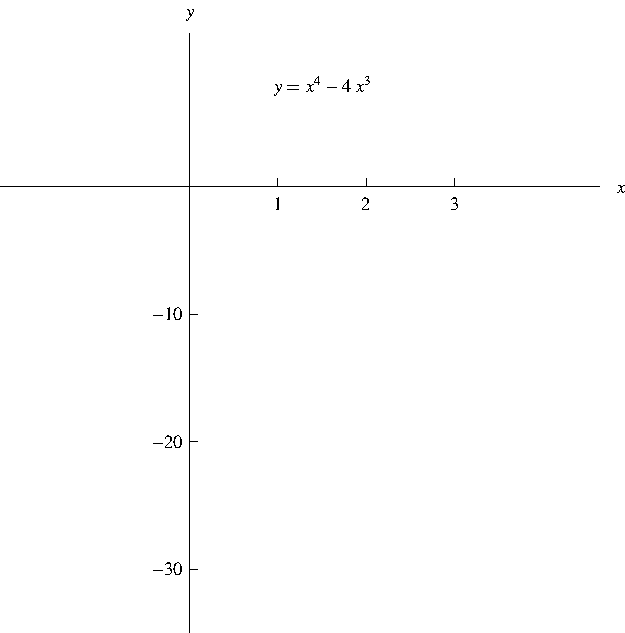
\includegraphics[height=4.5cm]{curve-sketching/pictures/04-03-ex6a.pdf}%
%}%
%\only<handout:0| 20-39>{%
%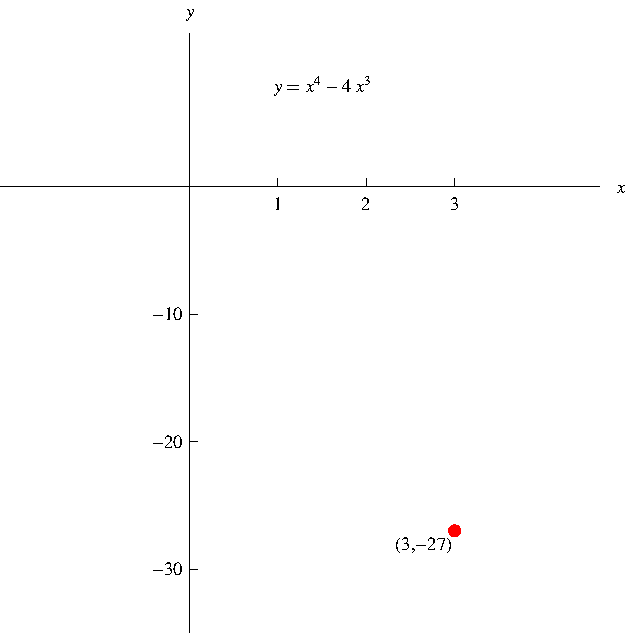
\includegraphics[height=4.5cm]{curve-sketching/pictures/04-03-ex6b.pdf}%
%}%
%\only<handout:0| 40-41>{%
%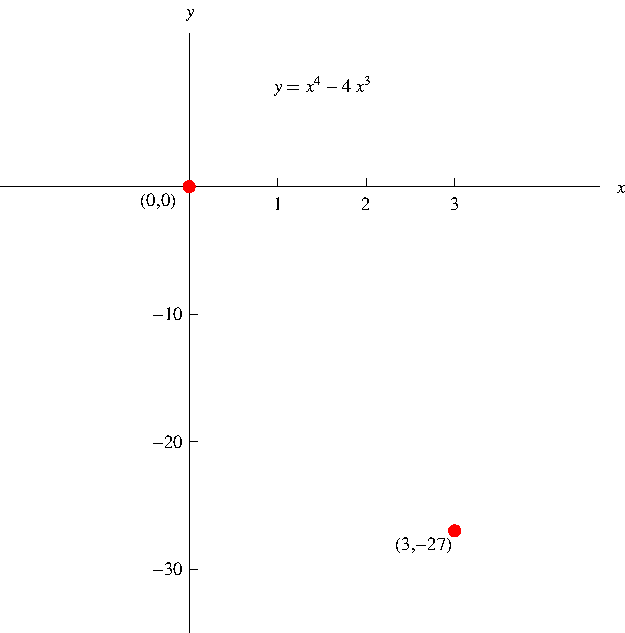
\includegraphics[height=4.5cm]{curve-sketching/pictures/04-03-ex6c.pdf}%
%}%
%\only<handout:0| 42-43>{%
%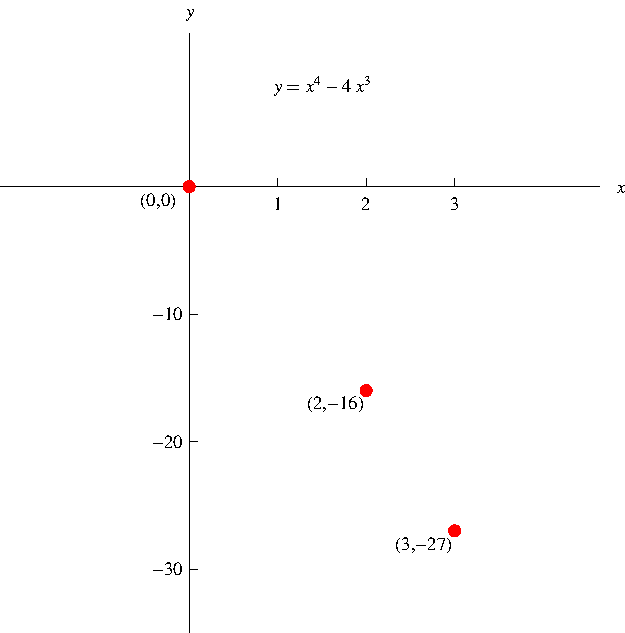
\includegraphics[height=4.5cm]{curve-sketching/pictures/04-03-ex6d.pdf}%
%}%
%\only<handout:0| 44-45>{%
%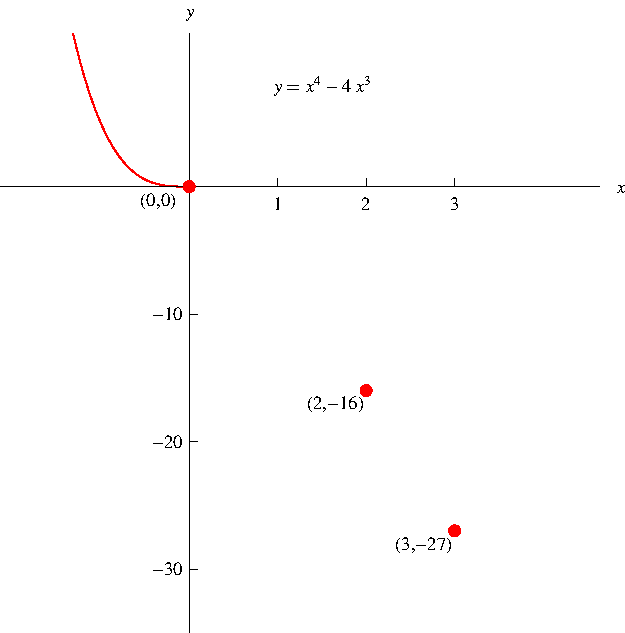
\includegraphics[height=4.5cm]{curve-sketching/pictures/04-03-ex6e.pdf}%
%}%
%\only<handout:0| 46-47>{%
%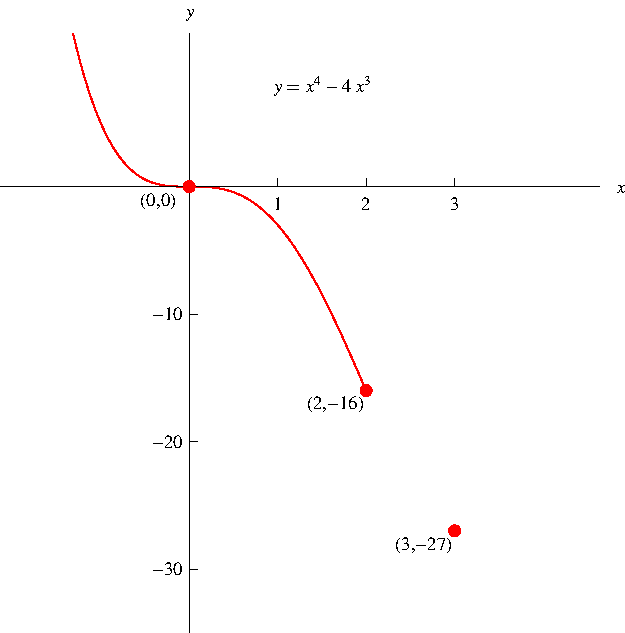
\includegraphics[height=4.5cm]{curve-sketching/pictures/04-03-ex6f.pdf}%
%}%
%\only<48->{%
%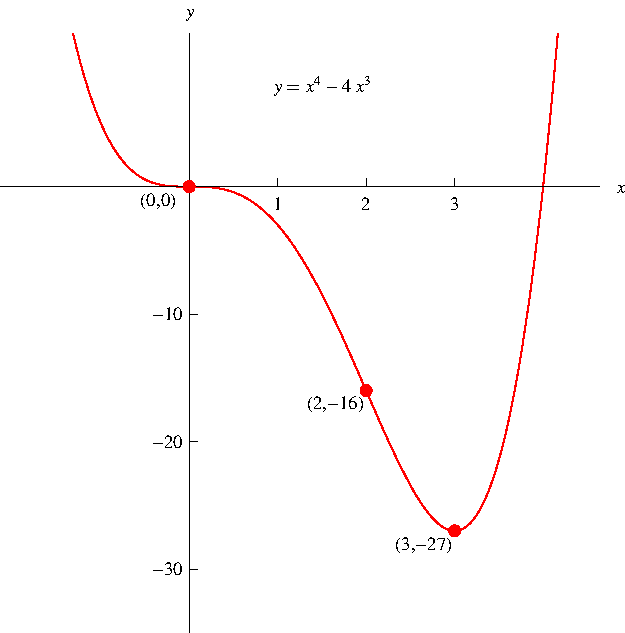
\includegraphics[height=4.5cm]{curve-sketching/pictures/04-03-ex6g.pdf}%
%}%

\vspace{.1in}

\uncover<28->{%
\ \ \ \begin{tabular}{|@{\ }r@{\ }|@{\ }c@{\ }|@{\ }l@{\ }|}
\hline
Interval & $f''(x)$ & \alert<handout:0| 35,43-48>{Concave}\\
\hline
\alert<handout:0| 29-30,37,43-44>{$(-\infty , 0)$} &%
\uncover<30->{\alert<handout:0| 30,37>{$+$}} &%
\uncover<35->{\alert<handout:0| 35,43-44>{up}}\\
\alert<handout:0| 31-32,37-38,45-46>{$(0, 2)$} &%
\uncover<32->{\alert<handout:0| 32,37-38>{$-$}} &%
\uncover<35->{\alert<handout:0| 35,45-46>{down}}\\
\alert<handout:0| 33-34,38,47-48>{$(2, \infty )$} &%
\uncover<34->{\alert<handout:0| 34,38>{$+$}} &%
\uncover<35->{\alert<handout:0| 35,47-48>{up}}\\
\hline
\end{tabular}
}%
\column{.58\textwidth}
\begin{itemize}
\item<2-| alert@2-3,23-26>  $f'(x) = $ \alert<handout:0| 4-5>{\uncover<3->{$4x^3 - 12x^2$} \uncover<4->{$ = $}\uncover<5->{$4\alert<handout:0| 11>{x^2}\alert<handout:0| 12>{(x-3)}$.}}
\item<2-| alert@6-7,29-34>  \alert<handout:0| 13-16>{$f''(x) = $} \alert<handout:0| 8-9>{\uncover<7->{\alert<handout:0| 13-16>{$12x^2 - 24x$}} \uncover<8->{$ = $} \uncover<9->{$12x(x-2)$.}}
\item<10->  Critical numbers: \uncover<11->{\alert<handout:0| 11,21-22>{$0$}} and \uncover<12->{\alert<handout:0| 12,17-18>{$3$}.}
\item<13->  \alert<handout:0| 13-14,21-22>{$f''(0) = \uncover<14->{0}$} and \alert<handout:0| 15-18>{$f''(3) =$ \uncover<16->{$36 > 0$.}}
\item<17->  Second Derivative Test:
\item<17-| alert@17-18>  \alert<handout:0| 47-48>{Local \uncover<18->{minimum} at $3$.}  \alert<handout:0| 19-20>{\uncover<19->{$f(3) =$ \uncover<20->{$-27$.}}}
\item<22-| alert@22>  No information about $0$.
\item<23->  First Derivative Test:
\item<23->  \alert<handout:0| 23-24>{$f'$ is \uncover<24->{$-$} on $(-\infty , 0)$} \alert<handout:0| 25-26>{and \uncover<26->{$-$} on $(0, 3)$}.
\item<27->  No local max or min at $0$.
\item<36->  Inflection points: \alert<handout:0| 39-40>{$\uncover<39->{(}\uncover<37->{\alert<handout:0| 37>{0}}\uncover<39->{,\uncover<40->{0})}$} and \alert<handout:0| 41-42>{$\uncover<39->{(}\uncover<38->{\alert<handout:0| 38>{2}}\uncover<39->{,\uncover<42->{-16})}$}
\end{itemize}
\end{columns}
\end{example}
\end{frame}
% end module curve-sketching-ex6

% begin module natural-exponential-ex7
\begin{frame}
\begin{example} %[Example 6, p. 277]
\begin{columns}[c]
\column{.4\textwidth}

\psset{xunit=0.5cm, yunit=0.5cm}
\begin{pspicture}(-5,-1)(5.5,10)
\psframe*[linecolor=white](-5,-1)(5.5,10)
\tiny
\psaxes[ticks=none, labels=none]{<->}(0,0)(-5,-1)(5,9.4)
\fcLabels{5}{9.4}
\fcXTickWithLabel{1}{$1$}
\fcXTickWithLabel{-1}{$-1$}
%Function formula: (e)^{(1)/(x)}
\uncover<6-20>{
\psplot[arrows=->, linecolor=\fcColorGraph, plotpoints=1000] {0.45} {0.55} {2.718281828 1 x div exp }
}
\uncover<20->{
\fcFullDot{-0.5}{0.135335283}
}
\uncover<10-20>{
\psplot[arrows=->, linecolor=\fcColorGraph, plotpoints=1000] {3.5} {5} {2.718281828 1 x div exp }
}
\uncover<21->{
\psplot[linecolor=\fcColorGraph, plotpoints=1000] {-5} {-0.01} {2.718281828 1 x div exp }
\psplot[linecolor=\fcColorGraph, plotpoints=1000] {0.45} {5} {2.718281828 1 x div exp }
\rput(2.3,3){$y=e^{\frac1x}$}
}
\uncover<10-20>{\psplot[arrows=->, linecolor=\fcColorGraph, plotpoints=1000] {-4.95} {-4} {2.718281828 1 x div exp }
}
\uncover<8-20>{
\psplot[linecolor=\fcColorGraph, plotpoints=1000] {-1.4} {-0.7} {2.718281828 1 x div exp }
\psplot[arrows=>-, linecolor=\fcColorGraph, plotpoints=1000] {-0.7} {-0.01} {2.718281828 1 x div exp }
}
\uncover<10->{
\psline[linecolor=\fcColorTangent, linestyle=dashed] (-4.95,1) (5,1)
\rput[t](4,0.9){$y=1$}
}
\end{pspicture}

%\ \only<handout:0| -5>{%
%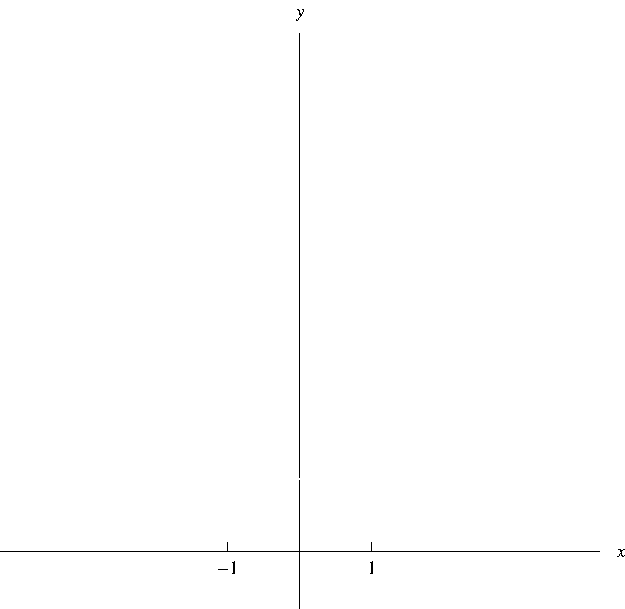
\includegraphics[height=5cm]{exponential-functions/pictures/07-02-ex7a.pdf}%
%}%
%\only<handout:0| 6-7>{%
%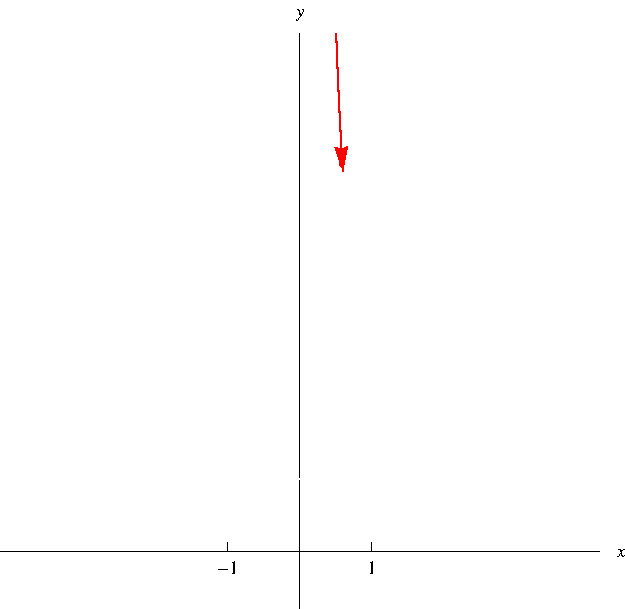
\includegraphics[height=5cm]{exponential-functions/pictures/07-02-ex7b.pdf}%
%}%
%\only<handout:0| 8-9>{%
%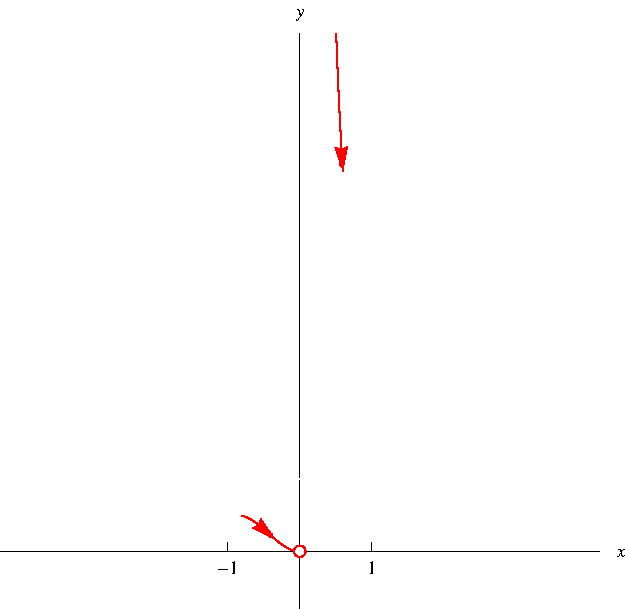
\includegraphics[height=5cm]{exponential-functions/pictures/07-02-ex7c.pdf}%
%}%
%\only<handout:0| 10-20>{%
%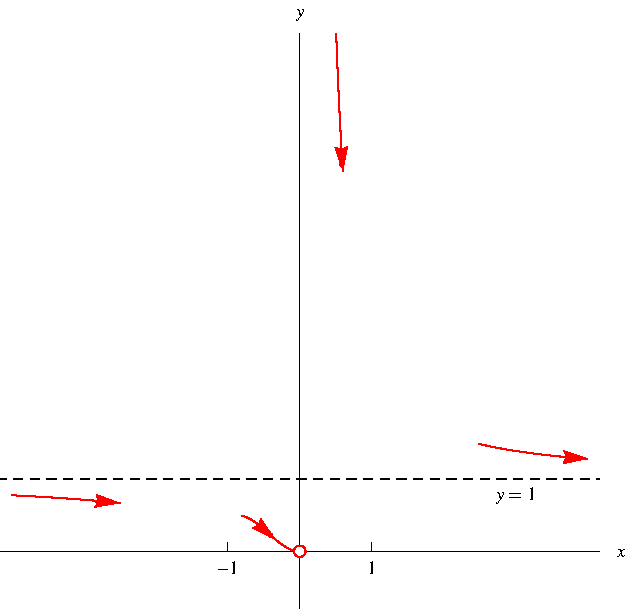
\includegraphics[height=5cm]{exponential-functions/pictures/07-02-ex7e.pdf}%
%}%
%\only<21->{%
%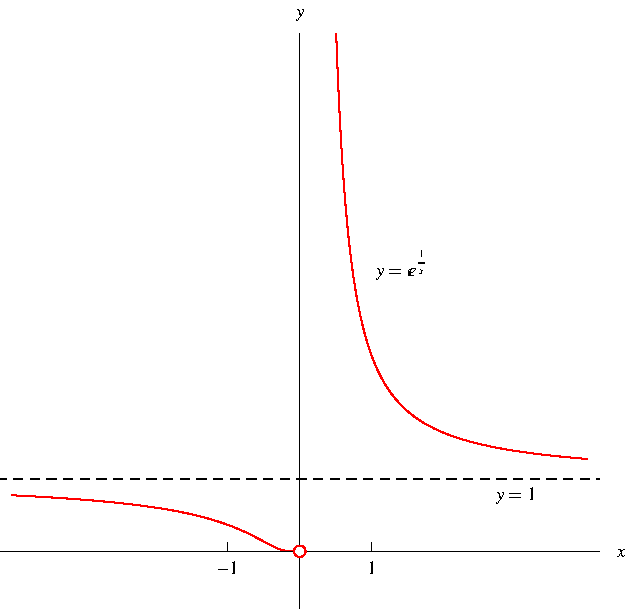
\includegraphics[height=5cm]{exponential-functions/pictures/07-02-ex7f.pdf}%
%}%
\column{.6\textwidth}
\qquad Draw the graph of $f(x) = e^{1/x}$.
\begin{itemize}
\item<2->  $f(x)$ is always positive.
\item<3->  Domain: everything but 0.
\item<4->  Check for vertical asymptote at 0.
\item<4->  $\displaystyle t = 1/x: \lim_{x\rightarrow 0^+} e^{1/x} \uncover<5->{ = \lim_{t\rightarrow\infty}e^t} \uncover<6->{ = \infty .}$
\item<4->  $\displaystyle t = 1/x: \lim_{x\rightarrow 0^-} e^{1/x} \uncover<7->{ = \lim_{t\rightarrow -\infty}e^t} \uncover<8->{ = 0.}$
\item<9->  As $x\rightarrow \pm \infty$, $1/x \rightarrow 0$.
\item<10->  Therefore $\lim_{x\rightarrow \pm \infty} e^{1/x} = 1$
\item<10->  $y = 1$ is a horizontal asymptote.
\end{itemize}
\end{columns}
\abovedisplayskip=0pt
\belowdisplayskip=0pt
\abovedisplayshortskip=0pt
\belowdisplayshortskip=0pt
\begin{align*}
\uncover<11->{f'(x) } & \uncover<11->{ = e^{1/x}\alertNoH{ 12-13}{(1/x)'}} \uncover<12->{ = e^{1/x}\alertNoH{ 12-13}{( \uncover<13->{-x^{-2}} )}} \uncover<14->{ = \alertNoH{ 17-18}{-e^{1/x}/x^2}.} \\
\uncover<15->{f''(x)} & \uncover<15->{ = -\frac{(x^2) ( - e^{1/x}/x^2) - (e^{1/x})(2x)}{x^4}} \uncover<16->{ = \alertNoH{ 19-20}{\frac{e^{1/x}(1+2x)}{x^4}}.}
\end{align*}
\alertNoH{ 18}{\uncover<18->{Always decreasing.}}  \alertNoH{ 20}{\uncover<20,21->{Inflection point: $(-1/2, e^{-2})$.}}
\end{example}
\end{frame}
% end module natural-exponential-ex7


% end lecture

\end{document}
